% Chapter Template

\chapter{Análisis de arquitecturas Clean, VIPER, Hexagonal} % Main chapter title

\label{Chapter2} % Change X to a consecutive number; for referencing this chapter elsewhere, use \ref{ChapterX}

\lhead{Capítulo 2. \emph{Clean vs VIPER vs Hexagonal}} % Change X to a consecutive number; this is for the header on each page - perhaps a shortened title
El objetivo principal de emplear una estructura fija para la implementación del proyecto es utilizar un único "lenguaje arquitectónico" familiar, tanto para el desarrollo de la aplicación en android, iOS o cualquier otra plataforma que pueda aparecer en el futuro, más bien durante la vida útil del producto. De esta manera no es necesario pagar un costo demasiado alto al incluir una implementación del mismo sistema para una plataforma distinta. 
Los desarrolladores de ambas plataformas podrán discutir aspectos de diseño, validar reglas de negocio y evacuar dudas sin tener en cuenta detalles de las platadormas, así mismo será más fácil conservar coherencia y mostrar armonía entre las implementaciones nativas para las plataformas.
%----------------------------------------------------------------------------------------
%	SECTION 1
%----------------------------------------------------------------------------------------

\section{Uncle Bob Clean Architecture}

También conocida como arquitectura de capas (onion architecture). El punto principal de este enfoque es que la lógica de negocio, también conocida como dominio, está en el centro del universo (Al medio entre las entradas del sistema y las salidas).
%\todo expandi esto negro
\section{Dominio Transparente}
Cuando se listen los directorios de un proyecto que cumple con los lineamiento de esta arquitectura, con tan solo leer el nombre de las carpetas debería ser posible casi de inmediato tener una idea de qué se trata esta aplicación, independientemente de la tecnología. Todo lo demás es un \emph{detalle de implementación}. \\
Por ejemplo, la persistencia es un detalle. Definir una interfaz con el objetivo de definir la responsabilidad con un contrato (Contrato de Persistencia),  de esta forma uno podría implementar de una manera rápida e inefieciente una estrategia de persistencia en memeoria RAM y no pensar en ello demsiadpo sino hasta que la lógica de negocio esté completamente definida. Una vez definidos los requerimeintos de persistencia y verificados con el cliente, se puede proceder a tomar una decisión definitiva de \textbf{cómo} deberán persistirse los datos.\\ 
Almacenamiento en una base de datos local, comunicación remota con un servicio REST remoto, almacenamiento sobre el sistema de archivos, ante este panorama incluso sería razonable pensar el planteo de la creación de un esquema de cache, y sin embargo no es poco frecuente que luego de la elicitación de requerimientos resulte que el sistema no tiene que persistir ningun resultado en absoluto.\\ 
En una frase: \textit{las capas internas contienen lógica de negocios, las capas externas contienen detalles de implementación}.
Adicionalmente esta arquitectura debe cumplir con un conjunto de características:

\begin{itemize}
	\item Regla de dependencia
	\item Abstracción
	\item Comunicación entre capas
\end{itemize}

\subsection{Regla de Dependencias}
La regla de dependencia se puede explicar mediante el siguiente diagrama:

\begin{figure}[htbp]
	\centering
	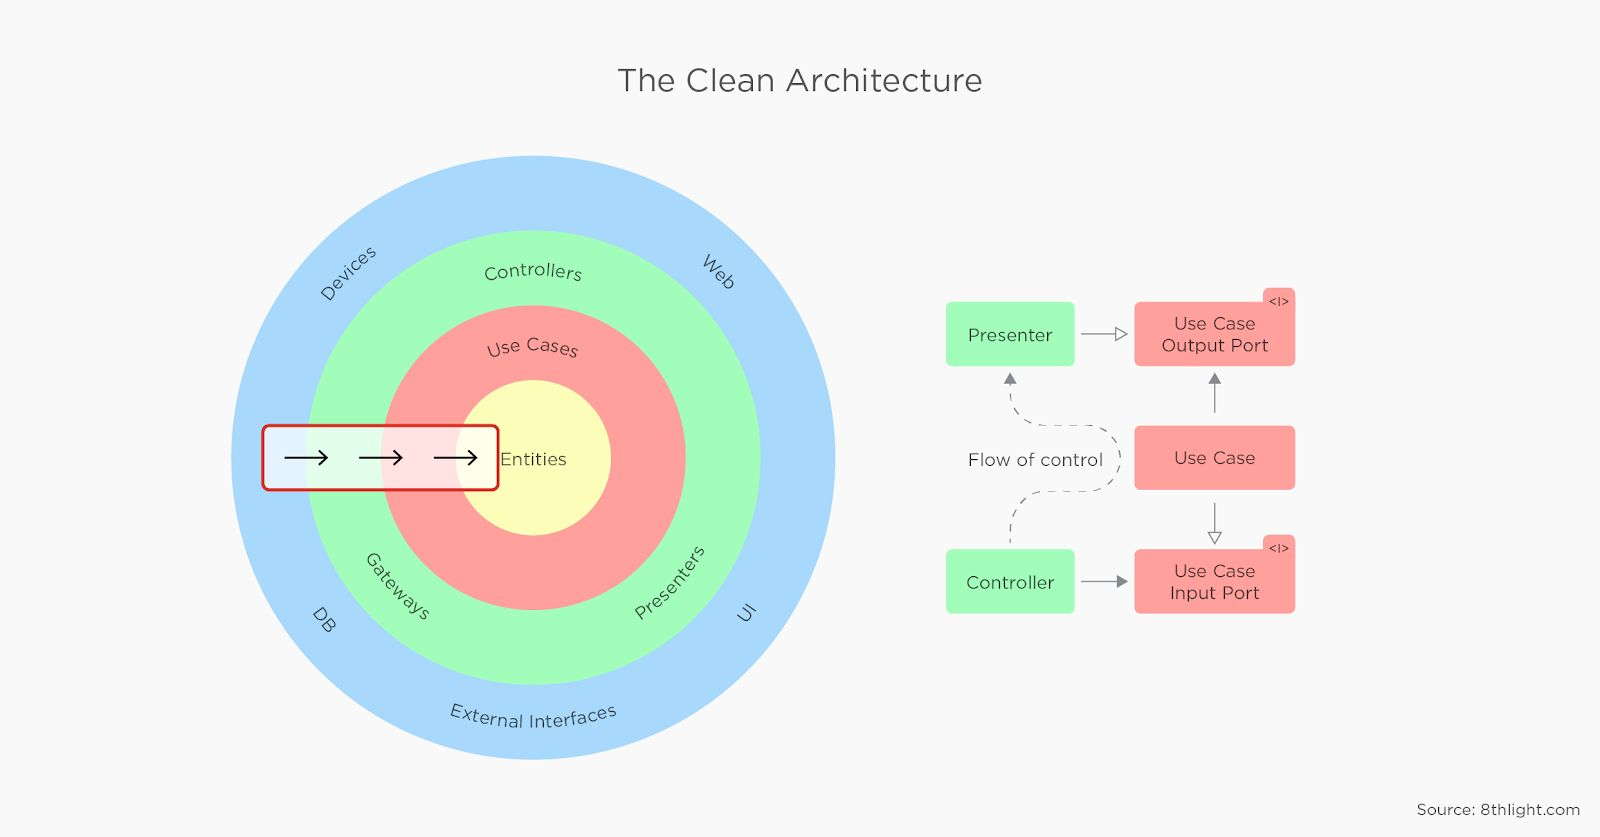
\includegraphics[width=1\textwidth]{Figures/-001.png}
	\rule{35em}{1pt}
	\caption[Principio de Dependecias]{Esquema de dependencias para una arquitectura en capas.}
	\label{fig:Diagrama_clasico}
\end{figure}


Las capas externas deben depender de las capas internas. Esas tres flechas en el cuadro rojo representan dependencias. En lugar de "depende", tal vez sea mejor usar términos como ''ve'', ''conoce'' o ''está consciente de...''. En estos términos, las capas externas ven, conocen y son conscientes de las capas internas, pero las capas internas no ven ni conocen, ni son conscientes de, las capas externas. Como dijimos anteriormente, las capas internas contienen lógica de negocios y las capas externas contienen detalles de implementación. Combinado con la regla de dependencia, se deduce que la lógica de negocio no ve, ni conoce, detalles de implementación. Y eso es exactamente lo que estamos tratando de lograr.

No existe una única forma de implementar esta regla dependerá del encargado del proyecto. Una estrategia consiste en colocar las clases de cada capa en paquetes diferentes, poniendo especial cuidado en no importar paquetes ''externos'' en paquetes ''internos''. Sin embargo, si algún programador del equipo no es consciente del principio de dependencias, nada les impediría romperlo. Un mejor enfoque sería separar las capas en diferentes módulos de Android, por ejemplo, y ajustar las dependencias en el archivo de construcción para que la capa interna simplemente no pueda utilizar la capa externa, sin embargo este enfoque implica un exaustivo conocimiento de la herramineta de construccion de la plataforma para la que se está desarrollando.

\subsection{Principio de Abstracción}
El principio de la abstracción ya se ha insinuado antes. Dice que, a medida que se están moviendo hacia el centro del diagrama, las cosas se vuelven más abstractas. Eso tiene sentido: como lo repetimos anteriormente el círculo interno contiene lógica de negocios y el círculo exterior contiene detalles de implementación.

\begin{figure}[htbp]
	\centering
	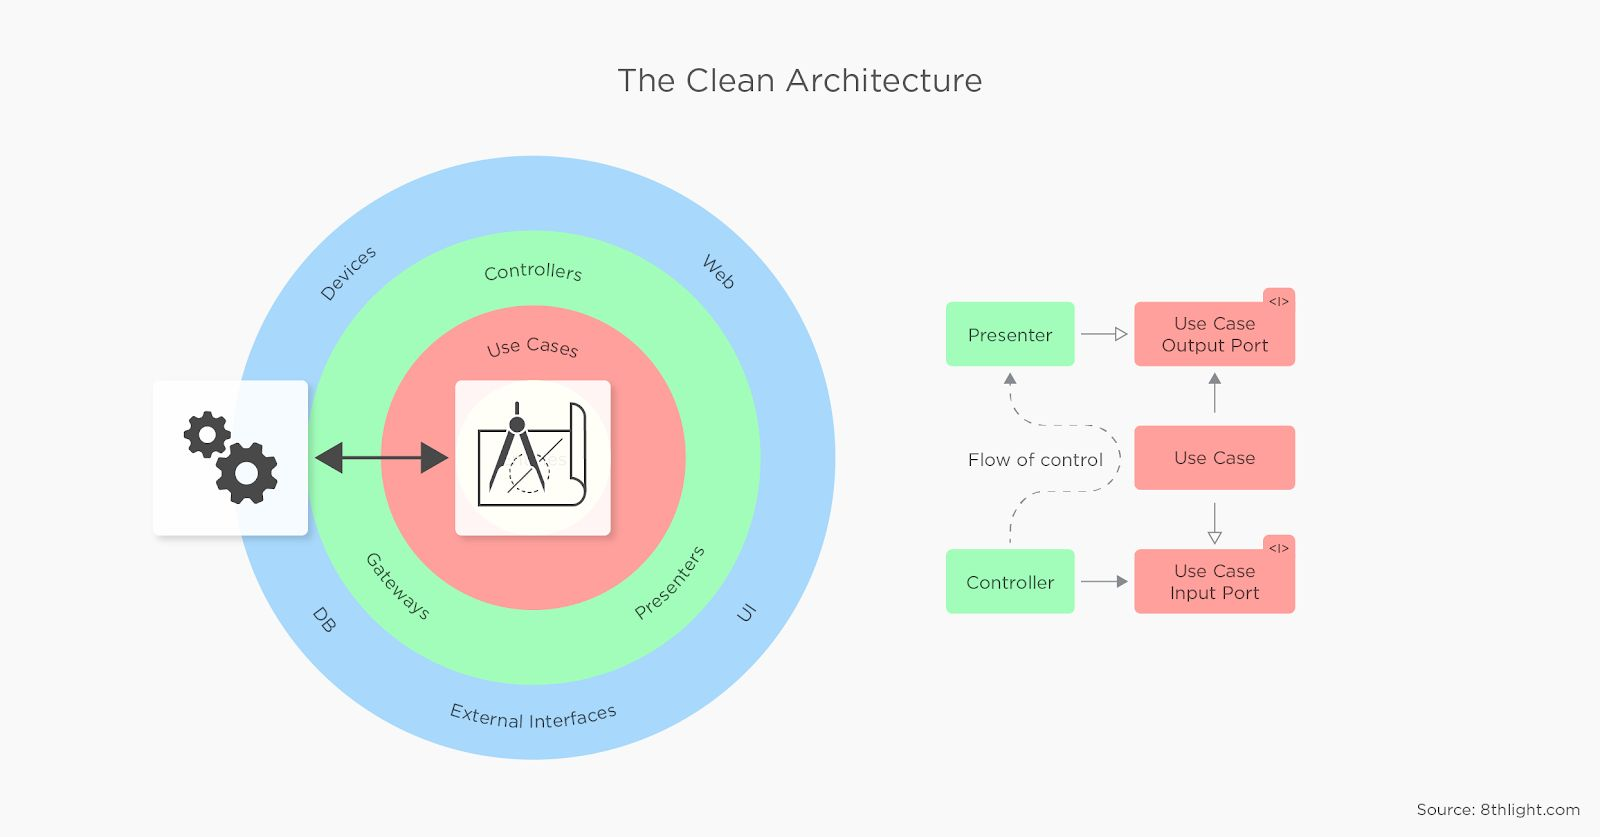
\includegraphics[width=1\textwidth]{Figures/-002.png}
	\rule{35em}{1pt}
	\caption[Abstraction Principle]{Principio de Abstracción en una arquitectura por capas.}
	\label{fig:C2_PA}
\end{figure}

Incluso puede plantearse el mismo componente lógico dividido entre varias capas, como se muestra en el diagrama. La parte más abstracta se puede definir en la capa interna, y la parte más concreta en la capa externa.

De esta manera, la lógica de negocios podría producir como un efecto secundario que se muestren notificaciones del sistema por ejemplo, pero no sabe nada acerca de los detalles de la implementación (cómo se implementan las notificaciones para una plataforma dada) . Además, la lógica empresarial ni siquiera sabe que existen detalles de implementación. Por lo tanto la regla de las dependencias se conserva.


\begin{figure}[htbp]
	\centering
	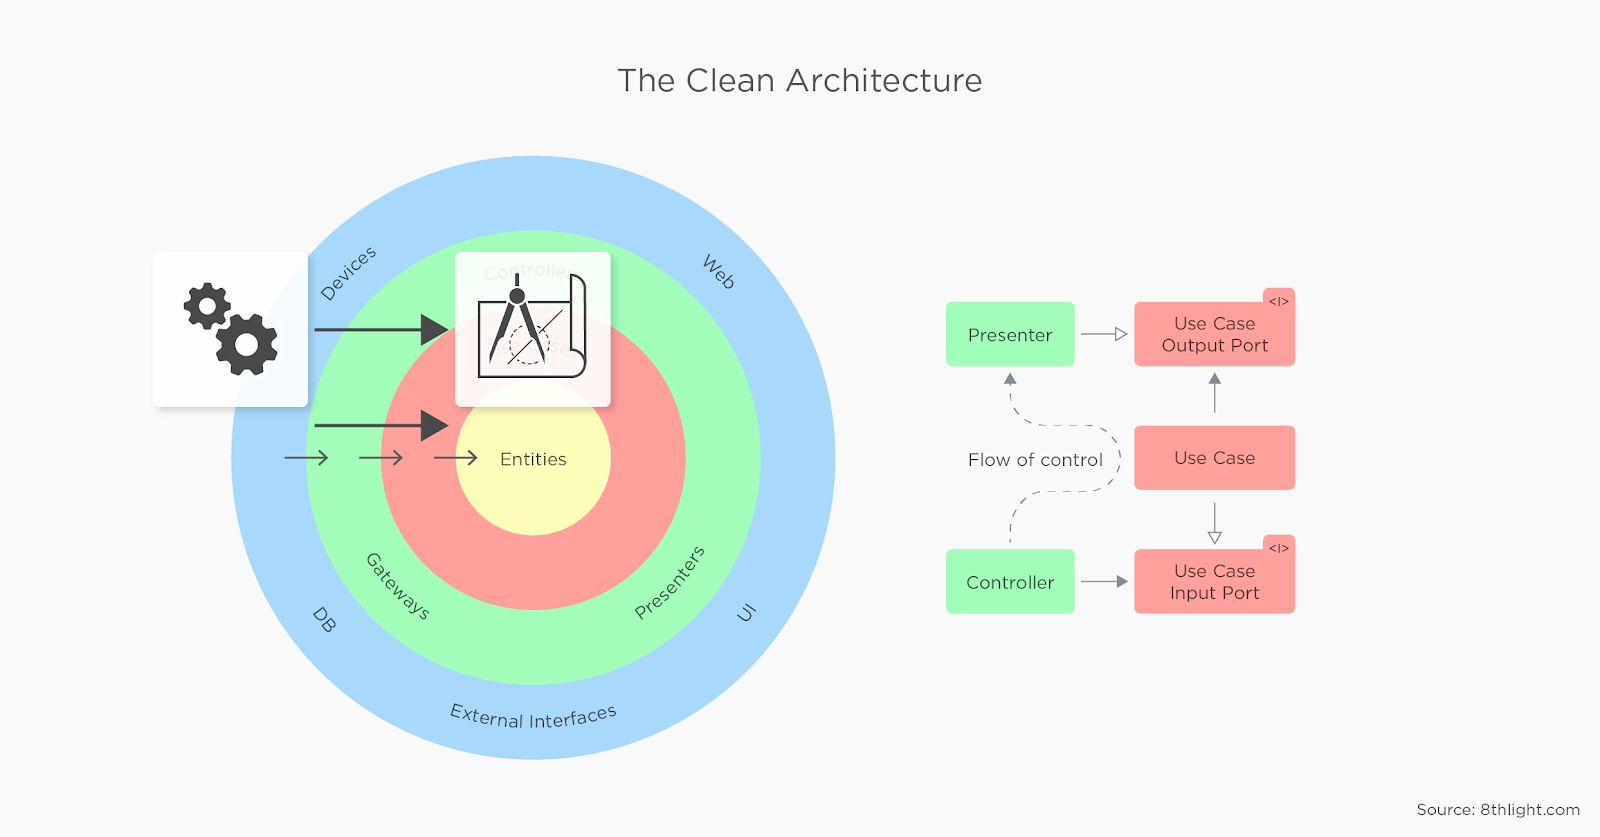
\includegraphics[width=1\textwidth]{Figures/-003.png}
	\rule{35em}{1pt}
	\caption[Abstraction Principle]{Principio de Abstracción en una arquitectura por capas.}
	\label{fig:C2_PA_02}
\end{figure}

\subsection{Comunicación entre Capas}
La lógica del negocio está en el medio y debe mediar entre los sitemas externos de salida y los sistemas externos de entrada como la interfaz de usuario, pero ni siquiera sabe que esos dos tipos existen. Esta es una cuestión de comunicación y flujo de datos. Necesitamos que los datos sean capaces de fluir de las capas externas a las internas y viceversa, pero la regla de dependencia no lo permite.

Sólo tenemos dos capas, la verde y la roja. El verde es exterior y sabe sobre el rojo, y el rojo es interior y sólo se conoce a sí mismo. Necesitamos que los datos fluyan desde el verde al rojo y viceversa. La solución ya se ha insinuado antes y se muestra en el siguiente diagrama:

\begin{figure}[htbp]
	\centering
	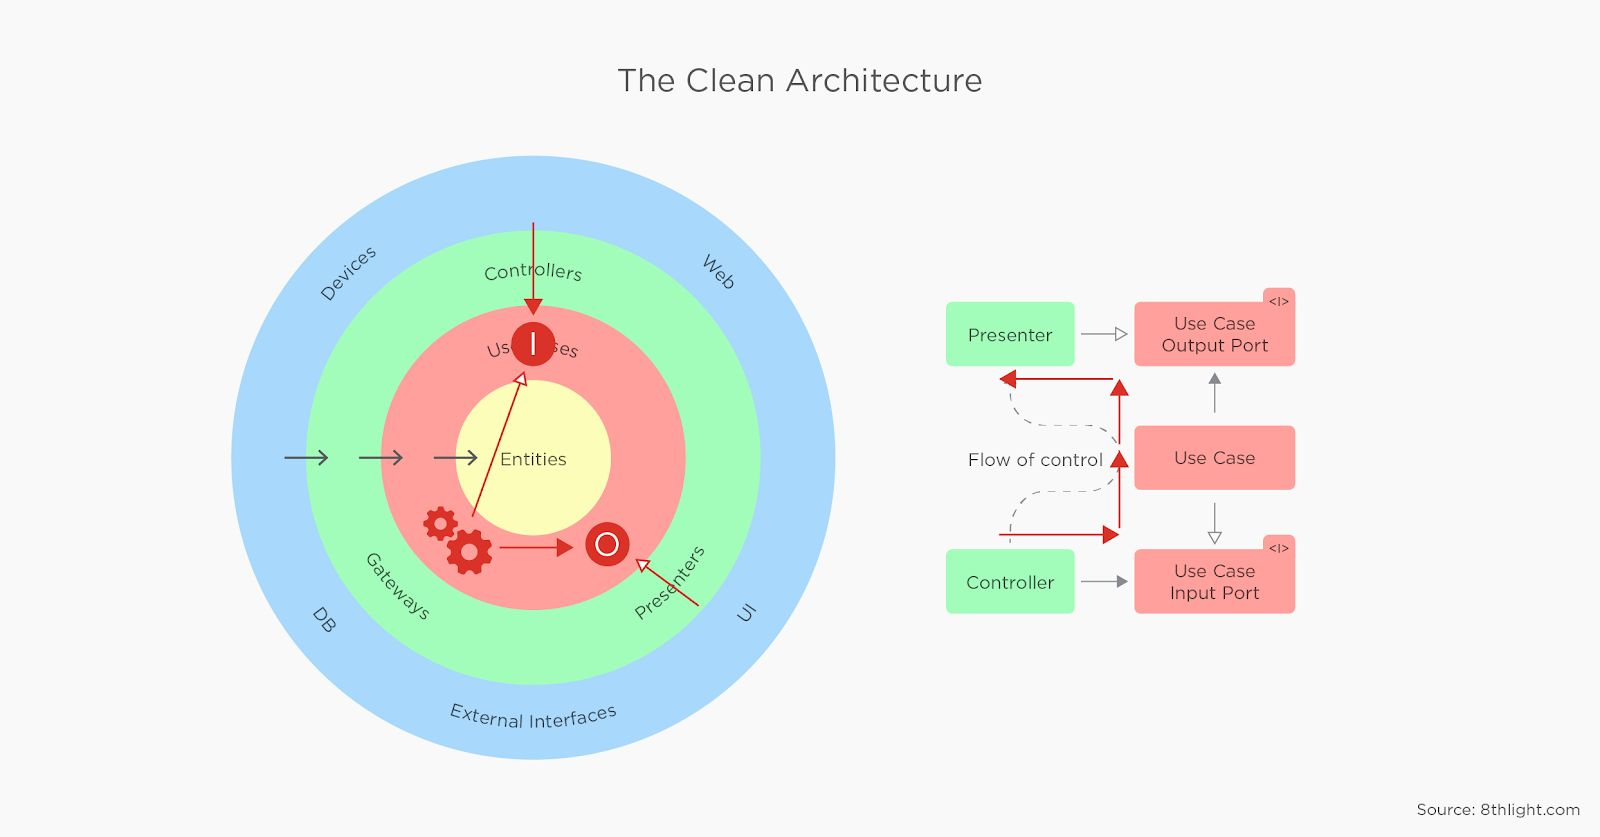
\includegraphics[width=1\textwidth]{Figures/-004.png}
	\rule{35em}{1pt}
	\caption[Layer Communication]{Comunicación entre capas.}
	\label{fig:C2_CC_01}
\end{figure}

La parte del diagrama en la parte inferior derecha muestra el flujo de datos. Los datos van desde el controlador, a través del puerto de entrada del caso de uso (o reemplazar el caso de uso con el componente de su elección), luego a través del propio caso de uso y después a través del puerto de salida del caso de uso al presentador.

El controlador tiene un puerto de entrada, literalmente tiene una referencia a él. Llama a un método en él, de modo que los datos van del controlador al puerto de entrada. Pero el puerto de entrada es una interfaz, y la implementación real es el caso de uso: por lo que ha llamado un método en un caso de uso y los flujos de datos al caso de uso. El caso de uso hace algo y quiere enviar los datos de vuelta. Tiene una referencia al puerto de salida, ya que el puerto de salida está definido en la misma capa, por lo que puede llamar al método en él. Por lo tanto, los datos van al puerto de salida. Y finalmente, el presentador es, o implementa, el puerto de salida.

\section{Arquitectura Hexagonal}
La arquitectura hexagonal comparte el enfoque de división de capas y utiliza los principios que la anterior sin embargo coloca a la DB en el centro del control del flujo de datos por lo que la diferencia real entre ambas es meramente de implementación y consideración.

\section{Arquitectura VIPER para iOS}
VIPER significa Views, Interactors, Presenters, Entities and Routing. La combinación de todos estos componentes vive dentro del llamado Módulo. La principal motivación detrás de esta arquitectura es proporcionar una solución a un problema en iOS conocido como Massive View Controllers. La arquitectura MVC tradicional utilizada para desarrollar la aplicación iOS simplemente no proporciona suficiente modularidad y separación de responsabilidades. Las partes View y Model permanecen más o menos limpias, pero toda la complejidad termina en ViewControllers, que tienen que manejar demasiadas cosas. Más de 1000 líneas de código no es poco común para un ViewController relativamente rico en funciones.

\begin{figure}[htbp]
	\centering
	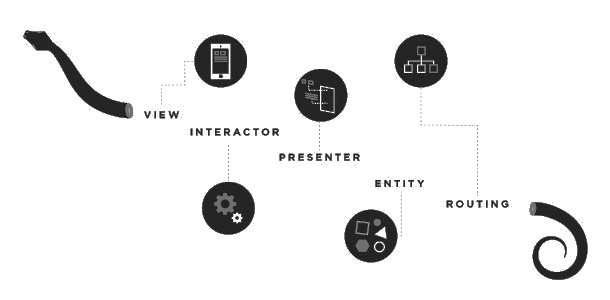
\includegraphics[width=1\textwidth]{Figures/-005_bw.png}
	\rule{35em}{1pt}
	\caption[VIPER Arch]{Esquema arquitectura VIPER.}
	\label{fig:C2S3_VA_01}
\end{figure}

Nuevamente se trata de una arquitectura separada por capas con separación de responsabilidades. En el caso de esta arquitectura en particular el único aspecto que cabe la pena hacer énfasis es en el esquema de comunicación que tiene lugar entre el Presentador y el Interactor. El Interactor trabaja con las Entidades y nunca las pasa al Presentador. En su lugar, los llamados objetos DisplayData se construyen a partir de las Entidades. Estos objetos contienen sólo los datos requeridos por el presentador que se mostrarán en la vista.

Hay un par de aspectos a los que uno debe prestar especial cuidado al utilizar la arquitectura VIPER en iOS. Lo primero es que uno tiene que instanciar todos los componentes con sus dependencias y hacer todo el cableado entre ellos en un módulo. Esto puede dar la impresión de que se está escribiendo demasiado del mismo código, cada vez que se crea un nuevo módulo, pero no hay forma de evitarlo. Es posible automatizar un poco este proceso escribiendo fragmentos de código personalizado y scripts de generación de código, pero muchas veces los resultados son demasiado generales para el módulo específico que estamos construyendo actualmente.

Otra aspecto difícil de manejar viene como resultado del cableado manual mencionado anteriormente - referencias cíclicas fuertes. Puesto que algunos de los componentes necesitan sus referencias cíclicas para trabajar, por ejemplo Presenter <-> Interactor, es posible generar memory leaks con gran facilidad si no se presta atención al momento de comunicar los objetos, cuáles referencias pueden ser fuertes y cuáles deben ser débiles. Esta tarea se vuelve más complicada cuanto más componentes y módulos hay en la aplicación. Es posible que se produzcan fugas adicionales de memoria ocultas cuando se usen características de lenguaje como los closures de Swift, así que uno debe ser muy cuidadoso al llamar a los métodos de Presenter desde un closure localizado dentro del Interactor.

Por último, esta estricta separación de las responsabilidades a veces conduce a tener Presenters muy simples, que sólo reorientar algunos flujos de datos de la Vista a los Interactores. Esto sucede cuando la arquitectura se aplica a unas pantallas relativamente simples, que no tienen muchas cosas que el Presentador pueda hacer.

\subsection{VIPER sobre Android}
\textit{La implementación de VIPER sobre android es impráctica y desbeneficiosa.}

Hay algunas diferencias significativas en la forma en que funcionan los SDK en iOS y Android. Android tiene Actividades, que son más o menos el equivalente de ViewControllers en iOS. Una gran diferencia es que uno no puede instanciar estos objetos. Uno puede pedirle al framework para iniciar una Actividad y luego puede anular sus métodos de ciclo de vida para hacer cualquier trabajo necesario. Por lo tanto, al implementar módulos VIPER, uno no puede realizar todo el cableado en una clase Wireframe cuando se instancia la actividad. En su lugar, todo el cableado del módulo VIPER inicial tiene que tener lugar cuando una Actividad es inicializada por el propio Framework. El SDK de Android también proporciona Fragmentos, que de hecho pueden ser instanciados por el programador, pero hay tanta magia relacionada con la creación de Fragmentos que el framework hace automáticamente, que hacen muy dificil controlar el ciclo de vida de tales Fragmentos. Por lo tanto, No considero el uso de Fragmentos como las vistas de VIPER e instanciándolas explícitamente en un Wireframe como una solución estable. Luchar contra el framework es siempre una mala idea.

Otra cosa específica en Android son los cambios de configuración, que normalmente destruyen toda la interfaz de usuario y la recrean. Eso incluye Actividades, Fragmentos y Vistas. Eso puede resultar catastrófico, porque todo el Módulo VIPER será eliminado por el recolector de basura (garbage colector) y recreado de nuevo. Así que uno tiene que asegurarse de que el estado de los componentes del módulo se guarda de alguna manera. Además, hay que tener cuidado con los objetos de larga vida y las operaciones de mantenimiento de las referencias a los componentes del módulo, ya que podría causar grandes fugas de memoria. Un ejemplo típico es una operación de petición de red, que tiene una referencia fuerte al Interactor del Módulo como su devolución de llamada. Dado que el Interactor tiene referencia al presentador y mantiene referencia a la vista, que contiene referencia a todas las cosas de la interfaz de usuario, esto podría dar lugar a una pérdida de memoria grande. Así que uno tiene que cuidar de limpiar tales referencias cuando un Módulo entero está siendo destruido y recreado.

Por estas razones se decidió descartar el uso de VIPER en el desarrollo de las apps como conseción y optar por implementar el enfoque de la Clean Architecture.


\newpage

